As soluções empregadas na fixação do motor ao robô e do Kinect ao motor foram satisfatórias pois a movimentação ficou suficientemente suave para sua possível utilização tanto na navegação autônoma quanto no mapeamento 3D. Por mais que o servo motor apresente erros ao manter sua posição este não foi suficiente para prejudicar as leituras do Kinect.

A utilização de interrupções no tempo para movimentar o motor foram essenciais para que o mesmo fizesse movimentos mais suaves, aperfeiçoando o controle de posição com o Wiimote. A Figura \ref{fig:kinectMontado} mostra o Kinect já acoplado ao motor e o motor ao robô.

\begin{figure}[H]
\centering
  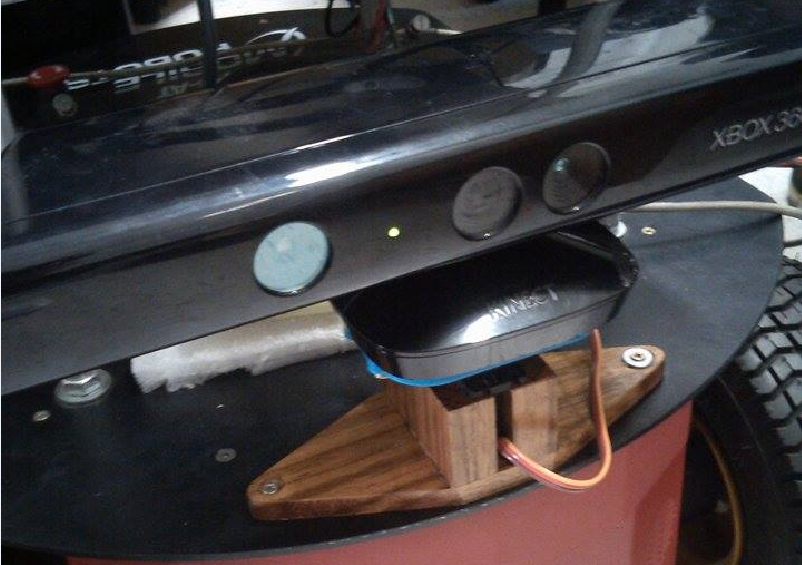
\includegraphics[scale=.35]{images/kinectMontado.png} \\
\caption{\small{Estrutura final de fixação do Kinect.}}
\label{fig:kinectMontado}
\end{figure} 